\documentclass{beamer}

\usepackage[utf8]{inputenc}
\usepackage{polski}
\usepackage{hyperref}
\usepackage{csquotes}
\usepackage{framed, color}
\usepackage{listings}

\definecolor{shadecolor}{RGB}{192, 192, 192}
\definecolor{Gray}{RGB}{64,64,64}
\definecolor{White}{RGB}{255,255,255}

\lstloadlanguages{Java}
\definecolor{mygreen}{rgb}{0,0.6,0}
\definecolor{mygray}{rgb}{0.5,0.5,0.5}

\lstset{ 
  backgroundcolor=\color{white},   % choose the background color; you must add \usepackage{color} or \usepackage{xcolor}; should come as last argument
  basicstyle=\footnotesize,        % the size of the fonts that are used for the code
  breakatwhitespace=false,         % sets if automatic breaks should only happen at whitespace
  breaklines=true,                 % sets automatic line breaking
  captionpos=b,                    % sets the caption-position to bottom
  commentstyle=\color{mygreen},    % comment style
  deletekeywords={},            % if you want to delete keywords from the given language
  escapeinside={\%*}{*)},          % if you want to add LaTeX within your code
  extendedchars=true,              % lets you use non-ASCII characters; for 8-bits encodings only, does not work with UTF-8
  firstnumber=1,                % start line enumeration with line 1000
  frame=none,	                   % adds a frame around the code
  keepspaces=true,                 % keeps spaces in text, useful for keeping indentation of code (possibly needs columns=flexible)
  %keywordstyle=\color{blue},       % keyword style
  language=Java,                 % the language of the code
  morekeywords={ enum },            % if you want to add more keywords to the set
  numbers=left,                    % where to put the line-numbers; possible values are (none, left, right)
  numbersep=5pt,                   % how far the line-numbers are from the code
  numberstyle=\tiny\color{mygray}, % the style that is used for the line-numbers
  rulecolor=\color{black},         % if not set, the frame-color may be changed on line-breaks within not-black text (e.g. comments (green here))
  showspaces=false,                % show spaces everywhere adding particular underscores; it overrides 'showstringspaces'
  showstringspaces=false,          % underline spaces within strings only
  showtabs=false,                  % show tabs within strings adding particular underscores
  stepnumber=1,                    % the step between two line-numbers. If it's 1, each line will be numbered
  tabsize=2,	                   % sets default tabsize to 2 spaces
  title=\lstname                   % show the filename of files included with \lstinputlisting; also try caption instead of title
}

\setbeamercolor{frametitle}{bg=Gray, fg=White}

\newcommand{\slideTitle}
{
	\frametitle{
		\small{
			\textbf{Narzędzia DevOps w chmurze Azure}
			}
		}
}

\newcommand{\source}[2]{
	\begin{flushright}
		\hfill {\scriptsize \href{#1}{#2}}	
	\end{flushright}
}

\begin{document}

\centering

% -----------------------

\begin{frame}
\frametitle{\textbf{}}

\textbf{
	\Huge{Narzędzia DevOps }
    \vskip 3mm
    \Huge{ w chmurze Azure}
}

\end{frame}

% -----------------------

\begin{frame}
\frametitle{\textbf{Rafał Pieńkowski}}

\begin{minipage}{0.45\textwidth}
\begin{center}
    \begin{itemize}
        \item Lead C\# Developer w Huuuge Games
        \item Staram się wprowadzać metodyki DevOps w moich projektach
        \item \vskip 2mm \hspace{10mm} 
\includegraphics[height=15mm]{logo.png}
        \item \vskip 2mm \hspace{10mm} 
\includegraphics[height=15mm]{astoria.png}
    \end{itemize}	
\end{center}
\end{minipage}
\begin{minipage}{0.45\textwidth}
    \hspace{15mm}
    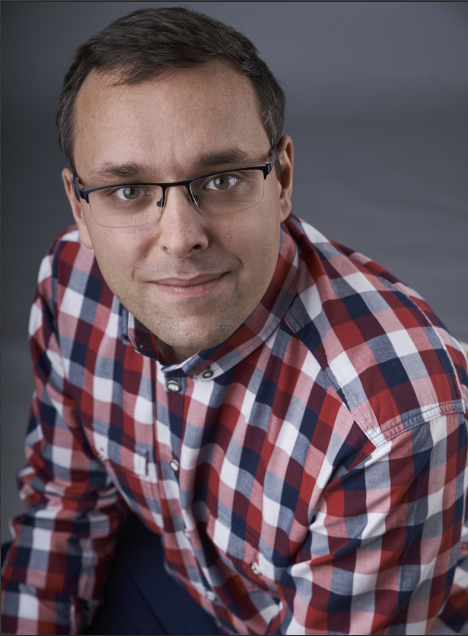
\includegraphics[height=5cm]{me.png}
\end{minipage}

\end{frame}

% -----------------------

\begin{frame}
\frametitle{\textbf{Społeczności}}

    
\includegraphics[width=\textwidth]{community.png}

\end{frame}
% -----------------------

\begin{frame}
\frametitle{\textbf{}}

\begin{minipage}{0.45\textwidth}
\begin{center}
    {\fontsize{30}{40}\selectfont \textbf{Historia}}
\end{center}
\end{minipage}
\begin{minipage}{0.45\textwidth}
    \hspace{15mm}
    \vskip 5mm
    
\includegraphics[height=35mm]{notebook.png}
    \source{https://undraw.co/illustrations}{undraw}
\end{minipage}

\end{frame}

% -----------------------

\begin{frame}
\frametitle{\textbf{}}

    
\includegraphics[height=25mm]{code_block.png} \\

    \scalebox{5}{$\Downarrow$} \\

    
\includegraphics[height=25mm]{server_down.png}
    \source{https://undraw.co/illustrations}{undraw}

\end{frame}
% -----------------------

\begin{frame}
\frametitle{\textbf{}}

    
\includegraphics[height=35mm]{aspnet-core.png}
    
\includegraphics[height=35mm]{cicd.png} \\
    
\includegraphics[height=35mm]{azure.png}

\end{frame}
% -----------------------

\begin{frame}
\frametitle{\textbf{}}

\begin{minipage}{0.45\textwidth}
\begin{center}
    {\fontsize{50}{60}\selectfont \textbf{Do \vskip 10mm pracy}}
\end{center}
\end{minipage}
\begin{minipage}{0.45\textwidth}
    \hspace{15mm}
    
\includegraphics[width=60mm]{working.png}
    \source{https://undraw.co/illustrations}{undraw}
\end{minipage}

\end{frame}
% -----------------------

\begin{frame}
\frametitle{\textbf{Linki}}

\begin{itemize}
    \item \href{https://docs.microsoft.com/en-us/azure/azure-resource-manager/templates/overview}{ARM Templates}
    \item \href{https://docs.microsoft.com/en-us/azure/app-service/}{App Service}
    \item \href{https://azure.microsoft.com/en-us/services/devops/}{Azure DevOps}
    \item \href{https://docs.microsoft.com/en-us/azure/azure-monitor/app/app-insights-overview}{Application Insights}
    \item \href{https://docs.microsoft.com/en-us/azure/storage/blobs/storage-blobs-introduction}{Azure Blob Storage}
    \item \href{https://github.com/rafalpienkowski/azure-devops-integration}{Github}
\end{itemize}	


\includegraphics[width=40mm]{qr-code.png}

\end{frame}
% -----------------------

\end{document}